\section{Components and Implementation} \label{sec:impl}

\begin{figure}[hbtp]
    \centering
    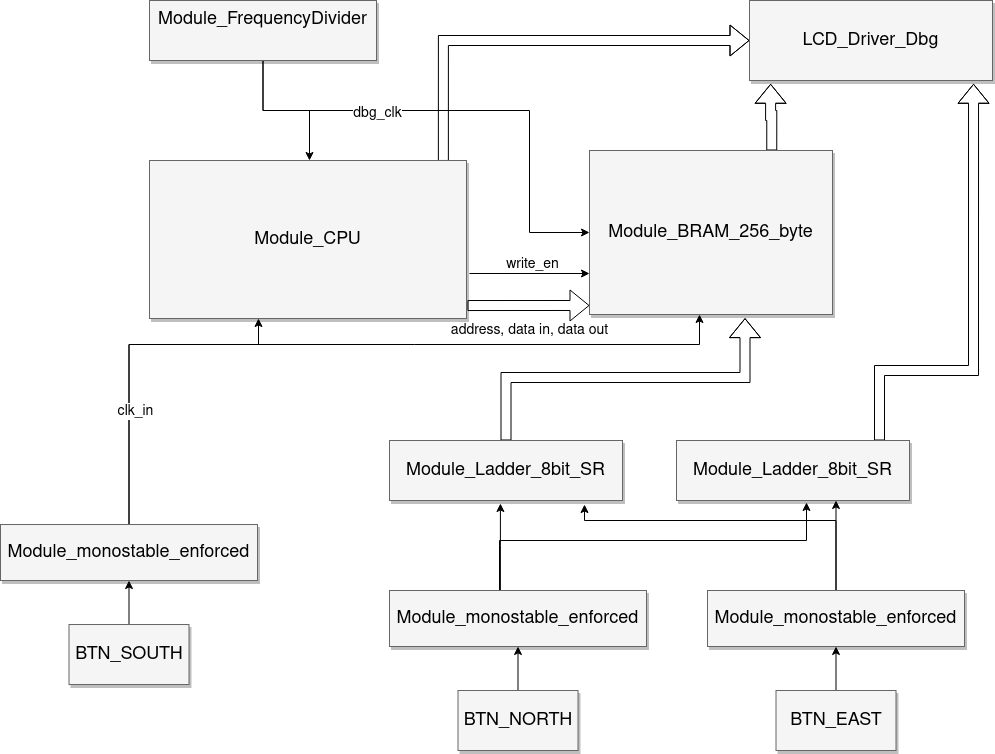
\includegraphics[width=0.9\textwidth]{img/System.png}
    \caption{Modules scheme of the computing system}
    \label{fig:system}
\end{figure}

The whole computing system is composed by three main modules: CPU, RAM and LCD debug modules
and by various other auxiliary modules.
The CPU comprises various 8-bit registers and uses them to fetch data from the RAM module, process it and, eventually, write back on the RAM.
The LCD Debug driver allows to access both the bytes stored in the RAM and the CPU registers from the LCD screen.
North and East pushbuttons are stabilized and used along with a switch to change the CPU registers or RAM values shown on the display.

Both the CPU and RAM run on three different clocks: a 50 MHz "Master" synchronization clock,
 a 1kHz debug clock used to comunicate with the LCD driver independently from the other operations
 and a last clock, sourced via the South pushbutton and used to govern the timing of the actual CPU and RAM operations.

 The RAM is pre-loaded with the data and instructions during the FPGA configuration phase.



\subsection{CPU Module}  \label{ssec:cpu}
\begin{figure}[hbtp]
    \centering
    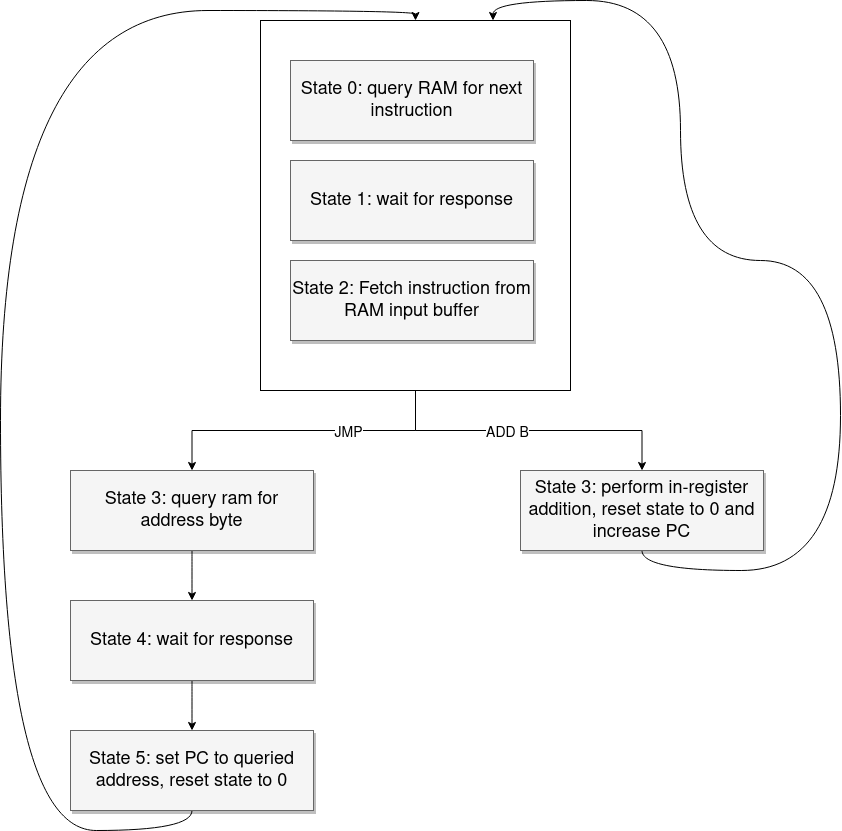
\includegraphics[width=0.7\textwidth]{img/States.png}
    \caption{Fetch-execute cycle corresponding to JMP and ADD instructions}
    \label{fig:diagram}
\end{figure}

The CPU module behaves like a state machine which fetches and executes one instruction at time from the RAM in the form of single-byte operation codes ("opcodes").
If the instruction requires it, the CPU can also fetch other bytes as parameters.
Each instruction execution is divided into several states, kept track by the \code{state} register.
Various other 8-bit registers are present to help store, process and write data.
At each \code{clk\_in} edge risetime, the module behaviour is determined by the current instruction and state.
When the last state corresponding to an instruction is reached, \code{state} register is reset to 0 and the process
restarts by fetching the next instruction.

In general, the instruction fetch-execution cycle behaves as follows:
\begin{itemize}
    \item \code{state} 0-2: The next instruction is fetched from the memory location pointed by the Program Counter (\code{PC}) and placed in the Instruction Register (\texttt{IR}).
    \item \code{state} 3- : The instruction is executed, eventually by reading or writing other bytes from memory or by operating on the internal registers. At the end, the \code{PC} address is incremented by one and \code{state} is reset to 0. The cycle then restarts
\end{itemize}

The following is a list of the internal CPU module registers:
\begin{itemize}
    \item \code{PC}: (8-bit) Program Counter, contains the memory address to the next instruction.
    \item \code{IR}: (8-bit) Instruction Register, Contains the byte corresponding to the current instruction in execution
    \item \code{A}: (8-bit) Accumulator, Register used to store fetched data and used by default as result recipient by the ADD instruction
    \item \code{B,C}: (8-bit) General purpose registers
    \item \code{W,Z}: (8-bit) Temporary registers for internal instruction operations, not directly accessible via instructions
    \item \code{H,L}: (8-bit) Registers used to store memory addresses, for instance used to write from register to referenced memory location
    \item \code{data\_addr,data\_out,write\_en}: Registers connected to output wirebuses, used to communicate read/write informations to RAM
    \item \code{flg\_carry,flg\_sign,flg\_zero,flg\_parity,flg\_auxiliary}: Various flags registers used to keep track of the results of the instructions.
    \code{flg\_auxiliary} is used as general-purpose flag to reduce the number of required instructions.
\end{itemize}

As a side note, the input/output operations usually require additional "buffering" times (blank states) to allow address informations delivery or data fetches.

\subsection{RAM Module}  \label{ssec:ram}
The \code{Module\_BRAM\_256\_byte} module \cite{BRAM} is based on the usage of the "Block Ram" modules present in the Xilinx Spartan 3A.
From the logical and Verilog code points of view, the Block RAM cells can be declared as arrays of $n$-bit registers.
In this specific module, the Block ram used is organized as an array of 256 8-bit memory cells, corresponding to a memory with 8-bit addresses.
The memory content is initialized using the Verilog command:
\begin{verbatim}
initial
begin
	$readmemh("memory.data", RAM, 0, 255);
end
\end{verbatim}
which prescribes how to load the RAM content from the file \code{memory.data} during the device configuration phase.

At each \code{clk\_in} tick, the RAM either reads or writes the content at address \code{addr} according to \code{write\_en}
by using the wires/registers \code{data\_in}, \code{data\_out}


\subsection{LCD driver Module}  \label{ssec:lcd}
The \code{LCD\_Driver\_Dbg} module is used to visualize the content of both the RAM module and the internal CPU registers.
The informations to be shown on display are inputed via the \code{addrInput, dataInput, CPU\_interface, dbg\_reg} wirebuses.
The user can select via switch one of the two devices, and further use the North and East buttons to move between the memory addresses
or CPU registers (implemented via a "Ladder" counter).
These informations are then passed to the here considered module via \code{addrInput} and \code{dbg\_reg}.

The LCD screen comprises a display data RAM used to store the shown characters,
and communicates with the FPGA board via the following lines:
\begin{itemize}
    \item \code{LCD\_DB}: an 8-bit "Data bit" wirebus. Here is used in 4-bit mode, therefore the lower 4 bits are set to high. 
    4-bit mode requires to perform all the operations by sending separately the upper and lower "nible" of each 8-bit word.
    \item \code{LCD\_E}: single-bit Read/write enable pulse, used to comunicate to the display that the other buses are ready for operating.
    \item \code{LCD\_RS}: single-bit register select, set to 1 only during display memory operations.
    \item \code{LCD\_RW}: read/write control, here permanetly set to 0 for write-only mode
\end{itemize}
Operating the LCD screen via Driver \cite{Board} requires the following steps:
\begin{itemize}
    \item Power-on initialization: initialization phase, the data bits are set and \code{LCD\_E} is pulsed according to required patterns and timings.
    \item Display configuration: Here multiple commands are issued to configure the device:
    \begin{itemize}
        \item Function set
        \item Entry mode set: address counter is set to auto-increment
        \item Display on, cursor and blinking are set off
        \item Clear Display
    \end{itemize}
    After issuing such commands, some time must be waited to allow the screen to function properly.
    \item Character writing: finally a cycle of character writing to the display RAM begins. For these commands, the \code{LCD\_RS} must be set
    to 1 and \code{LCD\_RW} to 0. Each character is represented by an 8-bit vlaue, and it must be transferred as indicated before, by sending first the upper nimble ant then the lower nimble.
    The writing address is then reset to the beginning and the process restarts.
\end{itemize}
The final output is:

\begin{verbatim}
    RM AA XX
\end{verbatim}
for the RAM debug mode, where AA stands for the 8-bit address and XX the relative value.
All bytes are represented in hexadecimal notation.

Foir the CPU debug the output is:
\begin{verbatim}
    CP RG XX
\end{verbatim}
where RG stands for a register name, and XX is the content.

Disclaimer: the LCD driver module here used is based on a modified version of code not originally writtend by the author.